\section{Durchführung}
\label{sec:Durchführung}
Der Versuchsaufbau ist schematisch in Abbildung \ref{fig:1} abgebildet.
Er besteht aus einer Halogenlampe, die Licht im nahen infrarot Bereich emittiert.
Dieses Licht wird durch eine Sammellinse zu einem parallelen Strahl gebündelt.
Dafür muss der Abstand zwischen Lampe und Linse genau der Brennweite der Linse entsprechen.
Als nächstes passiert der Lichtstrahl einen Lichtzerhacker, der auf etwa 450 Hz eingestellt ist. 
Dadurch wird das Licht in Impulse gesplittet. Diese Lichtmpulse treffen dann 
auf ein Glan-Thompson-Prisma, wodurch sie linear polarisiert werden. 
Anschließend trifft das Licht auf die GaAs-Probe, welche sich in 
der Symmetrieebene eines Elektromagneten befindet und für Licht im infrarot Bereich transparent ist.
Der Elektromagnet ist an ein Konstantstromgerät angeschlossen und erzeugt so ein 
zeitlich konstantes Magnetfeld.
Hinter dem Elektromagneten sind Interferenzfilter aufgebaut, 
wodurch nur eine Wellenlänge beobachtet werden kann und welche austauschbar sind. 
Hinter diesen Filtern befindet sich ein zweites Glan-Thompson-Prisma, 
dieses spaltet das Licht in zwei senkrecht zueinander polarisierte Strahlenbündel auf. 
Jedes der beiden Strahlenbündel wird durch eine Sammellinse auf einen Photowiderstand fokussiert.
Die Widerstände sind an einen Differenzverstärker angeschlossen, welcher wiederum an einen 
Selektivverstärker angeschlossen ist. Der Selektivverstärker ist auf die Frequenz des 
Lichtzerhackers eingestellt. Als letztes Element ist ein Oszilloskop angeschlossen, welches 
als Nulldetektor genutzt wird, um zu überprüfen, wann die Intensitäten der beiden aufgespaltenen 
Lichtbündel gleich sind.

\begin{figure}[H]
    \centering
    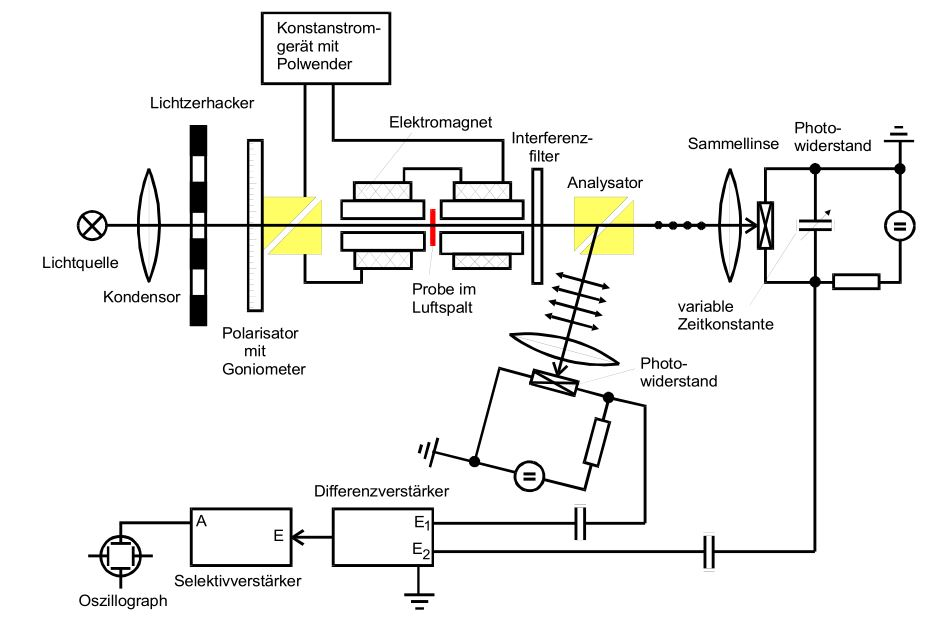
\includegraphics[width=1\textwidth]{Aufbau.jpg}
    \vspace{-10pt}
    \caption{Schematischer Aufbau des Versuchs \cite{Anleitung}.}
    \label{fig:1}
\end{figure}

Zu Beginn des Versuchs wird die Apperatur justiert. Zudem wird überprüft, ob durch drehen des Glan-Thompson-Prismas, 
also des Polarisators, bei jedem der beiden aufgespaltenen Lichtbündel eine Nullamplitude erreicht werden kann. 
Als erste Probe wird eine n-dotierte GaAs-Platte in den Elektromagneten eingesetzt. 
Diese Probe hat eine Dicke von L = 1,36 mm mit N = 1,2$\cdot 10^{18}$ cm$^{-3}$. Der erste Interferenzfilter 
mit $\lambda = 1,06 \: \mu$m. Die Spannung des Elektromagneten wird auf das Maximum von 10 V erhöht, 
der Polarisator gedreht, bis das Minimum der Intensitätsdifferenz der beiden Strahlenbündel auf dem Oszilloskop 
zu erkennen ist. Anschließend wird der Winkel $\Theta$ am Polarisator abgelesen.
Die Spannung des Elektromagneten wird auf null runter geregelt, der Elektromagnet wird umgepolt 
und sie Spannung wird wieder auf 10 V erhöht. Anschließend wird wieder das Minium auf dem Oszilloskop gesucht und 
$\Theta$ abgelesen. Diese Prozedur wird für die anderen acht Interferenzfilter bis zu einer Wellenlänge 
von $\lambda = 2,65 \: \mu$m wiederholt.
Diese Messungen werden mit der anderen n-dotierten GaAs-Probe mit der Dicke L = 1,296 mm und N = 2,8$\cdot 10^{18}$ cm$^{-3}$, 
sowie einer hochreinen GaAs-Probe der Dicke L = 5,11 mm, für alle neun Interferenzfilter wiederholt.
Anschließend wird mittels einer Hallsonde die magnetische Flussdichte des Elektromagneten vermessen. 
Dafür wird die angelegte Spannung auf die maximalen 10 V eingestellt. 
Dann wird die Magnetische Flussdichte über 3 cm hinweg, in der Mitte des Magneten, jeden Millimeter gemessen.

